\documentclass[../Main.tex]{subfiles}
\begin{document}
Chapter 3 will provide a thorough examination of the system characteristics and architecture of our novel social login system. This chapter provides a fundamental understanding of the complex mechanisms and distinguishing characteristics that set our system apart in the decentralized oracle network field. Next, the chapter will provide a detailed description of the system architecture. The social login system has been divided into three sub-processes to enhance clarity and address its inherent complexity. This section will provide a comprehensive explanation of each sub-process, emphasizing its distinct functionalities and responsibilities within the overall system flow. By breaking down the system into separate phases, readers can understand the specific steps required to process a user's request and smoothly execute the social login mechanism.
\section{System's characteristics}
This study examines the efficacy and adaptability of a system that utilizes conventional social login methods to augment the UX of DApps. The following characteristics can be more detailed: \\
\indent\textbf{Security} - combining the potential benefits of blockchain smart-contract, SSS, and Pedersen DKG protocol. The security infrastructure of the system is established upon the utilization of blockchain smart contracts. Programmable contracts, operating on a decentralized network, guarantee the attributes of transparency, immutability, and tamper-proof execution of operations. Shamir secret sharing is used to fortify the protection of cryptographic keys and other forms of private information. This method entails breaking up a secret into smaller pieces and giving them to several parties. The Petersen DKG protocol distributes and secures cryptographic key generation, ensuring system security. This system lets a group of people generate a shared cryptographic key without anyone having the full key. 

\indent\textbf{Efficacy and adaptability} - By leveraging blockchain's decentralized nature, Web3Auth eliminates the reliance on centralized identity providers, reducing the potential for single points of failure and enhancing security. Additionally, blockchain-based identity systems enable instant verification of user credentials, eliminating the need for lengthy verification processes and reducing transaction times. The open solution's architecture enables seamless integration with any DApps, making it easier for developers to adopt and implement with their products. 

\indent\textbf{User-friendly} - This solution supports popular authentication mechanisms such as social login which are widely used in the traditional web. This familiarity allows users to leverage their existing accounts and authentication methods, reducing the learning curve and providing a seamless transition into the Web3 space. Users can easily authenticate their identities across multiple DApps using a unified and standardized protocol, without the need to remember and manage multiple usernames and passwords. This eliminates the hassle of creating and maintaining numerous accounts, making the user experience more streamlined and efficient.

\indent\textbf{Scalability} - Compatible with any type of social authentication, including Facebook, Google, and Twitter. Utilizing a decentralized architecture increased the request's performance and volume by spreading it across multiple executors and parallel handling processes.
\newpage
\section{Overall of system}
\begin{figure}[H]
 \centering
 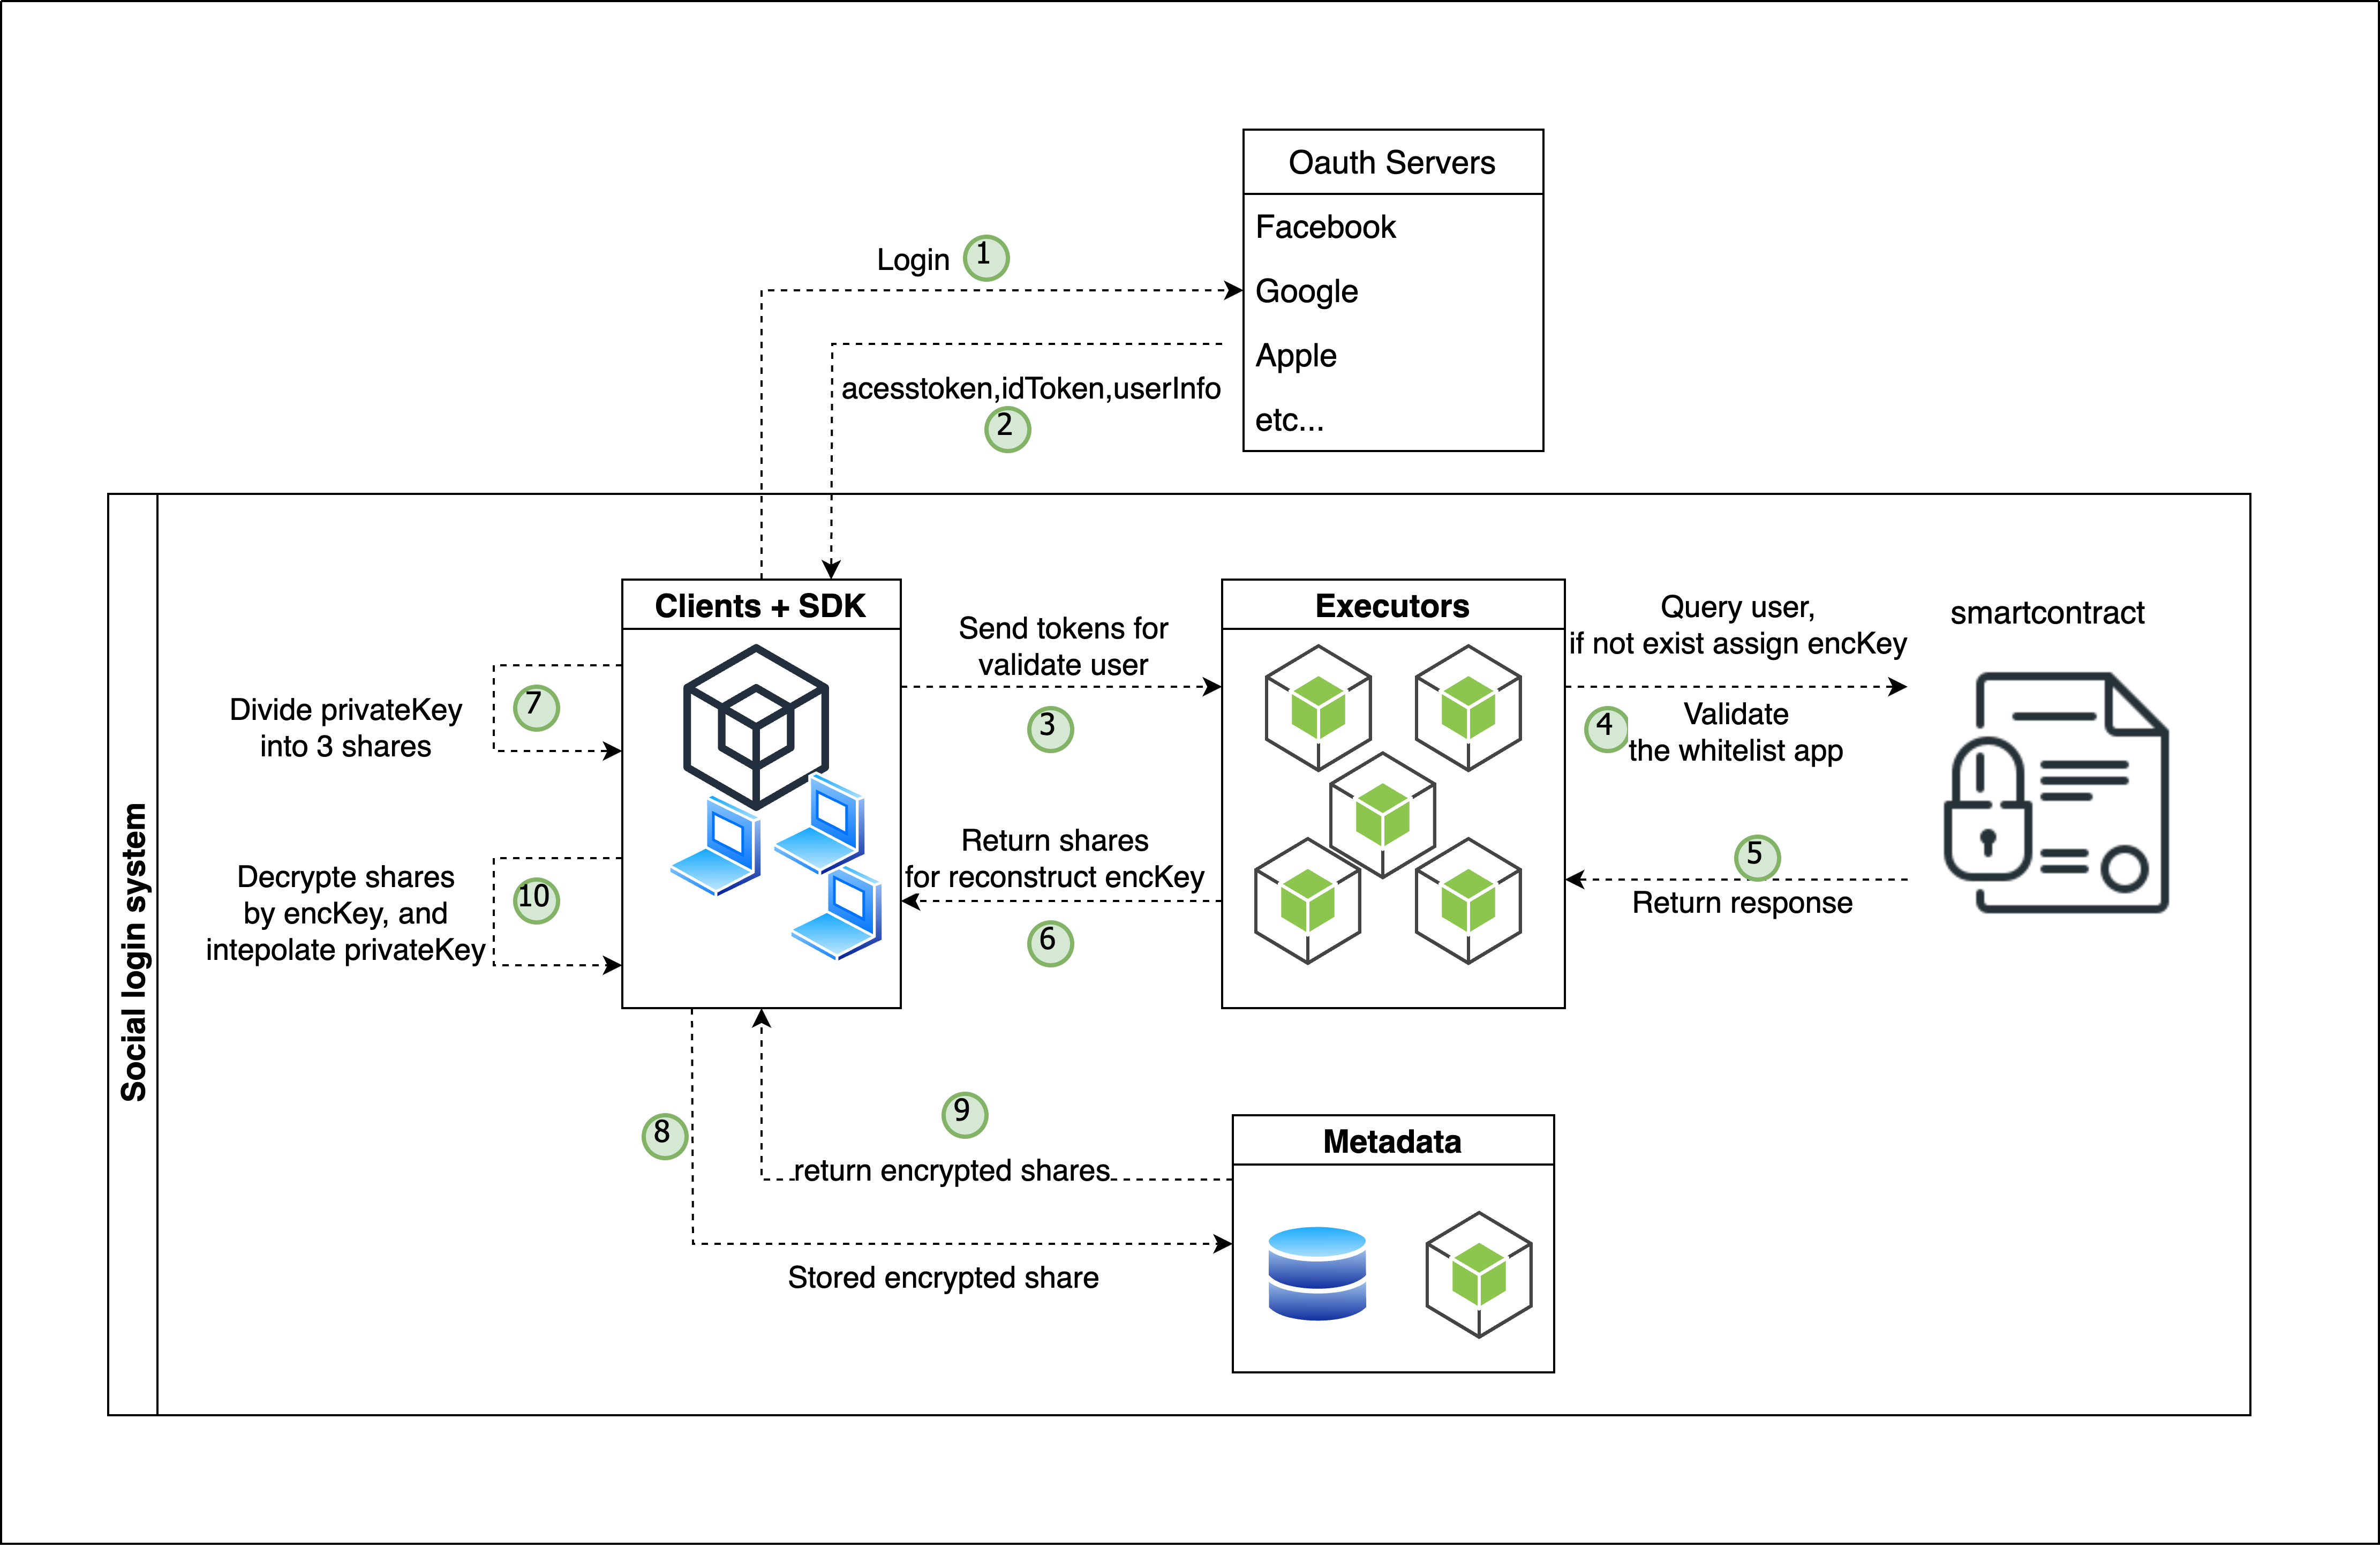
\includegraphics[scale=0.1]{Figure/OverallSocialLoginSystem.png}
    \caption{Overall the system}
    \label{fig:OverallSystem}
\end{figure}
Figure \ref{fig:OverallSystem} depicts the exhaustive and intricate request flow of a user interacting with the social login system. This intricate process has been meticulously subdivided into three distinct sub-processes, each with a specific function, to facilitate a clearer and more comprehensive comprehension of the system's overall functionality and interactions. The user's voyage begins when they initiate a request, at which point they choose the convenience and security of the social login feature. Subsequently, the initial sub-process begins, meticulously validating the user's input and ensuring the request's highest level of security. This validation phase is essential for protecting against potential vulnerabilities and maintaining the system's integrity. After the request has successfully passed the initial validation phase, the second sub-process authenticates the social logon credentials against the relevant provider's robust authentication system. This crucial phase ensures the authenticity of the user's identity and restricts system access to only authorized individuals. The rigorous authentication procedure protects against unauthorized access and fosters a secure environment for user interactions. The third sub-process assumes control upon successful authentication of the social logon credentials, orchestrating the logic for constructing the encryption key and the assignment key. These keys are essential to assuring the security and confidentiality of user information throughout their interaction with the system. The encryption key ensures that sensitive information remains confidential and protected from potential breaches, while the assignment key optimizes the user experience by facilitating the seamless assignment of roles and permissions. Throughout this complex process, the system employs smart contracts and blockchain technology, which serve as the foundation for preserving and protecting user data for the duration of the blockchain's active state. By leveraging the capabilities of smart contracts and blockchain, the system maintains a decentralized and transparent infrastructure, thereby nurturing user confidence.


\subsection{Auth0 connection}
\begin{figure}[H]
 \centering
 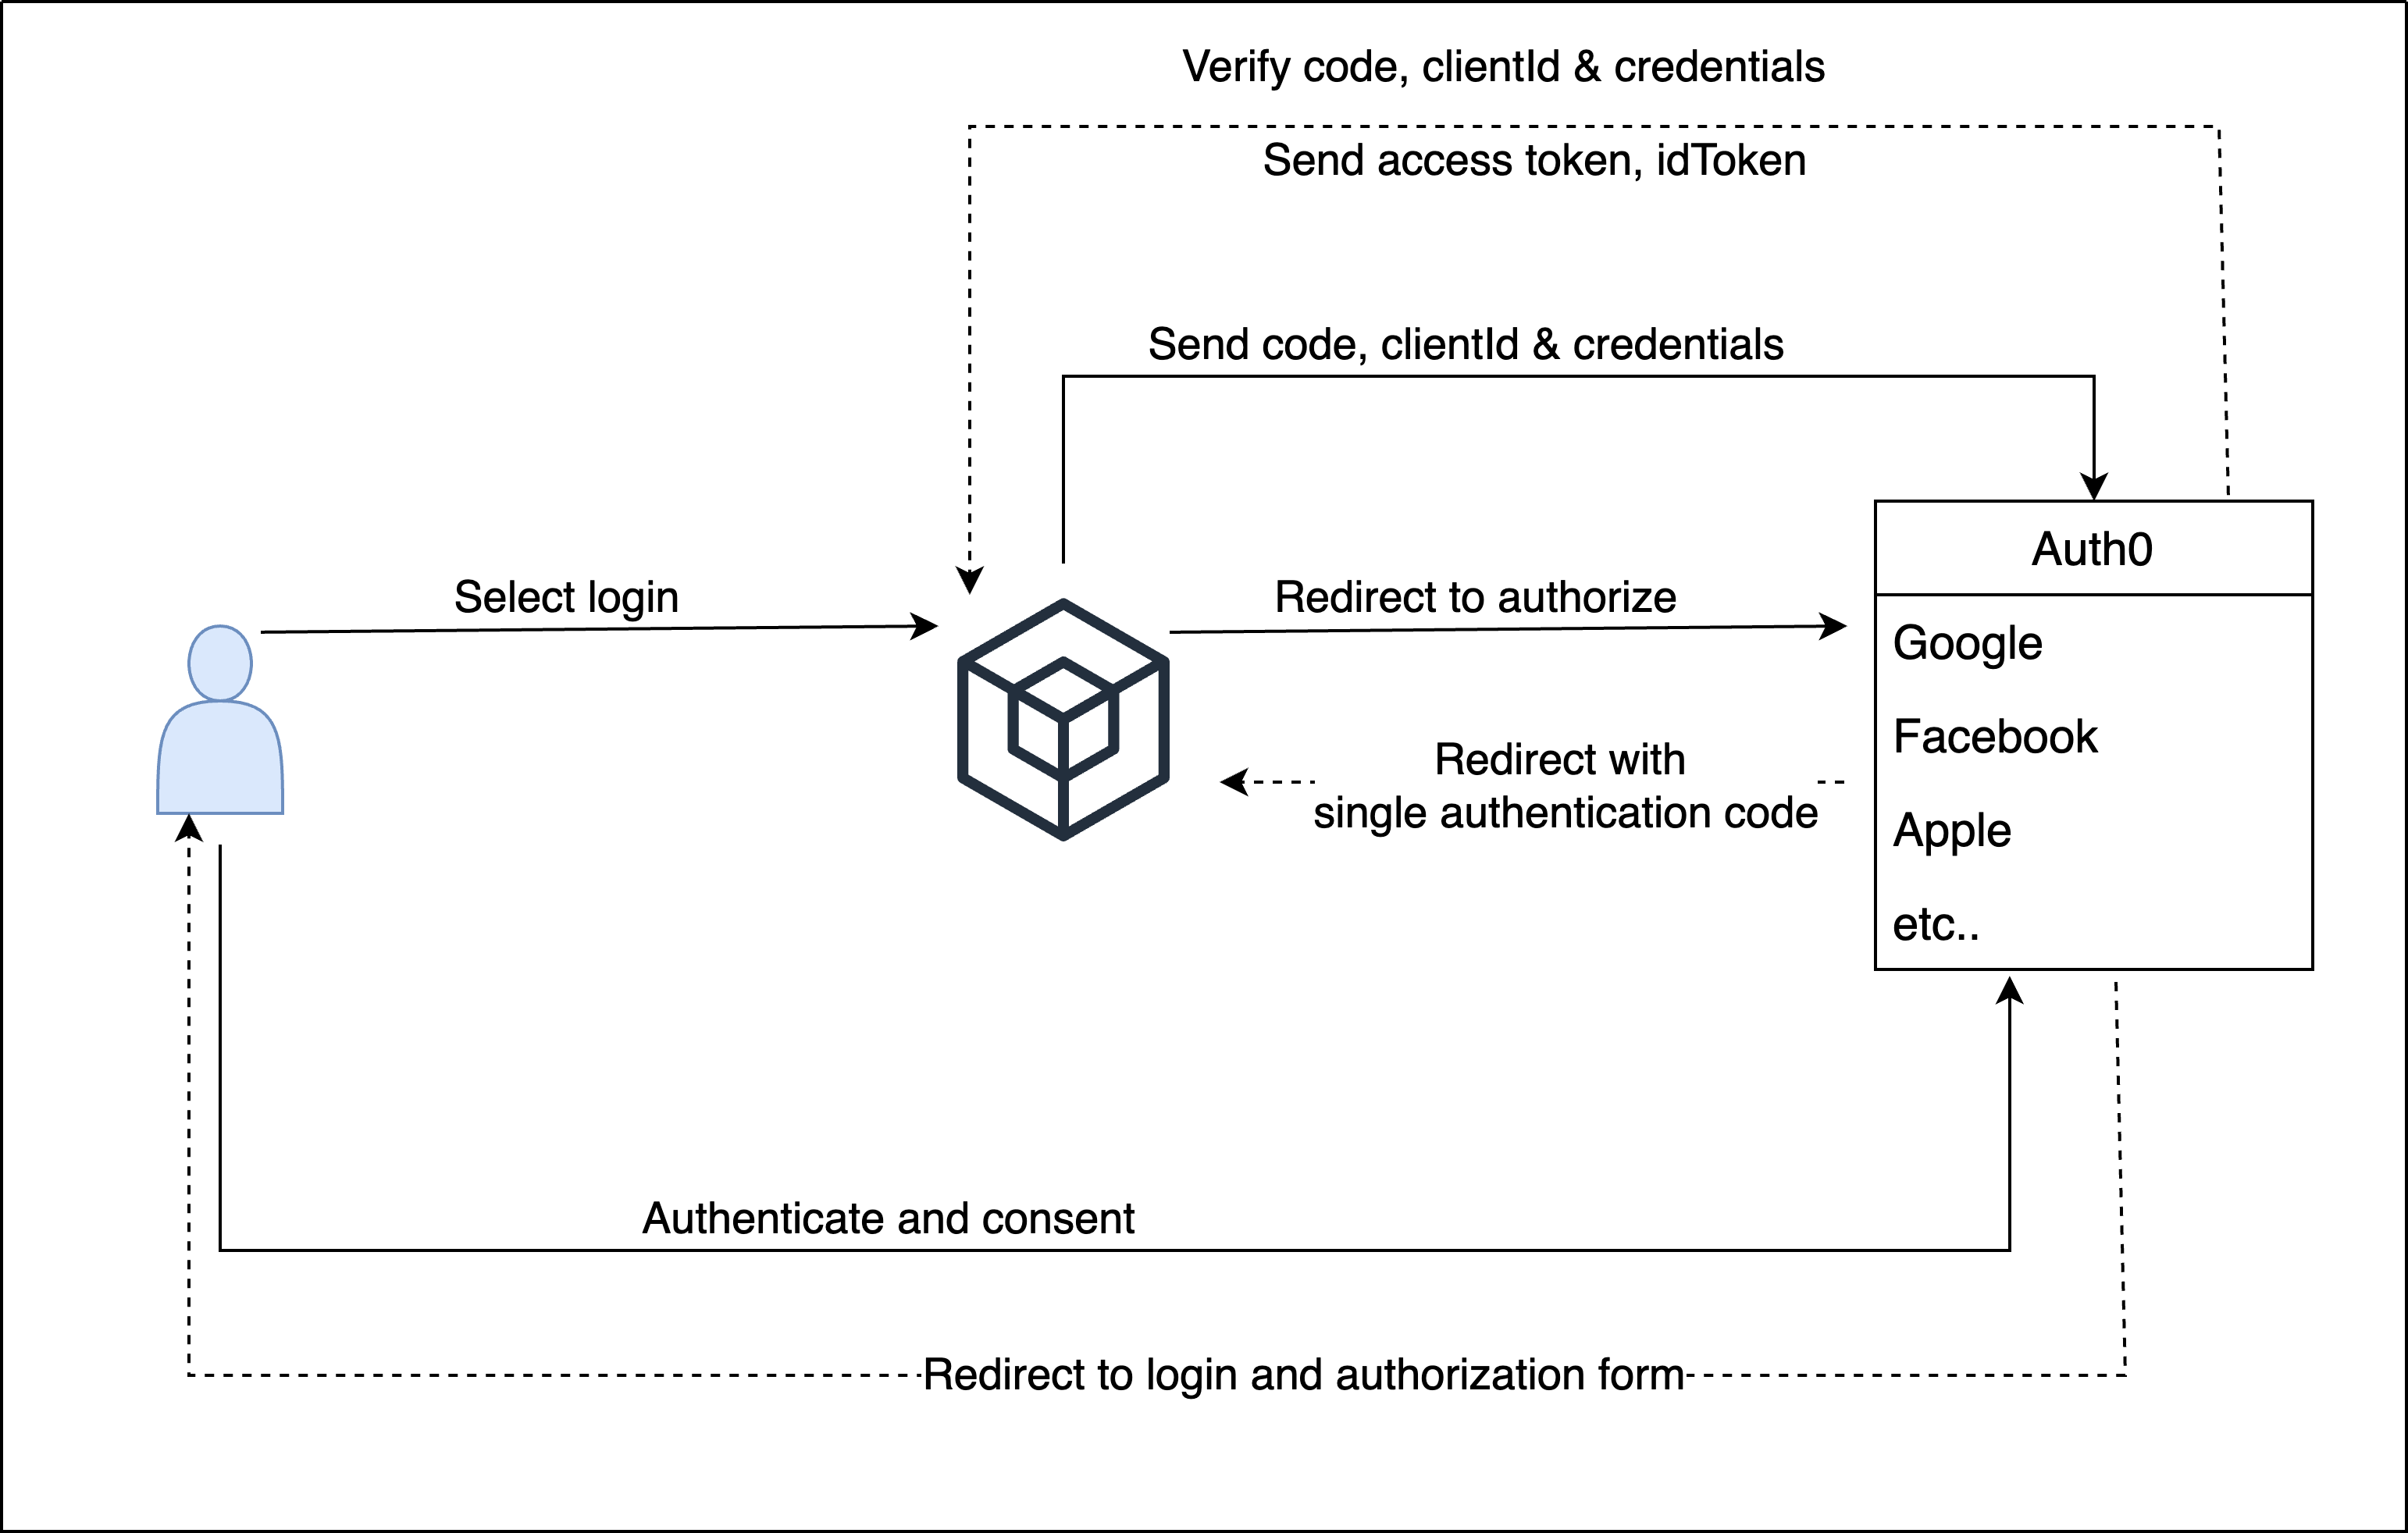
\includegraphics[scale=0.14]{Figure/Oauth-connection.png}
    \caption{Auth0 connection}
    \label{fig:Auth0-connection}
\end{figure}
Figure \ref{fig:Auth0-connection} provides a comprehensive graphical representation of the Auth0 authentication and authorization solution, highlighting its critical role in facilitating secure and streamlined user interactions within the application. When a user decides to authenticate within the application, they are presented with a number of options, including traditional username and password authentication and social registration via Google or Facebook. This versatility enables users to select their preferable authentication method, thereby enhancing the overall user experience. The application initiates the authentication process by redirecting the user to Auth0's authorization endpoint once the user has selected the authentication type. This phase begins the secure process of user authentication and authorization. At the authorization endpoint, the user is presented with a login and authorization prompt, where they authenticate themselves securely and grant the required permissions. This step ensures that only authorized users have access to the application's resources and can perform particular operations, thereby protecting the application's integrity and sensitive data. The Auth0 server redirects the user back to the application with an authorization code following successful authentication and assent. This authorization code is a crucial component of the subsequent authentication and authorization processes. The application then exchanges this authorization code along with its own credentials and client ID with the token endpoint of Auth0. The Auth0 server meticulously verifies this exchange, ensuring the authenticity and validity of the supplied data. Upon successful authentication, the Auth0 server issues the application both an access token and an ID token. During the authentication and authorization procedure, these tokens serve unique functions. The access token functions as proof of authorization, allowing the application to authenticate future requests on behalf of the user. It grants access to protected resources and API endpoints, facilitating secure and seamless application-to-server communication. The access token is typically included in API request parameters by the application, facilitating secure data exchange and interactions. The ID token, on the other hand, comprises vital user information, which facilitates identification and authentication within the application. It may contain information such as the user's email address, identify, and other pertinent attributes. The ID token enables the application to recognize the user and customize the user's experience within the application, thereby creating a personalized, user-centric environment. Auth0 is a highly dependable and efficient authentication and authorization solution due to its extensive feature set and stringent security measures. Auth0 assures the confidentiality and integrity of user data throughout the entire authentication and authorization procedure by adhering to secure protocols and industry best practices. Its seamless integration with multiple authentication methods and customizable user experiences make it a valuable asset for application developers seeking to improve the security and usability of their software.
\subsection{Requesting encKey for Executors}
\begin{figure}[H]
 \centering
 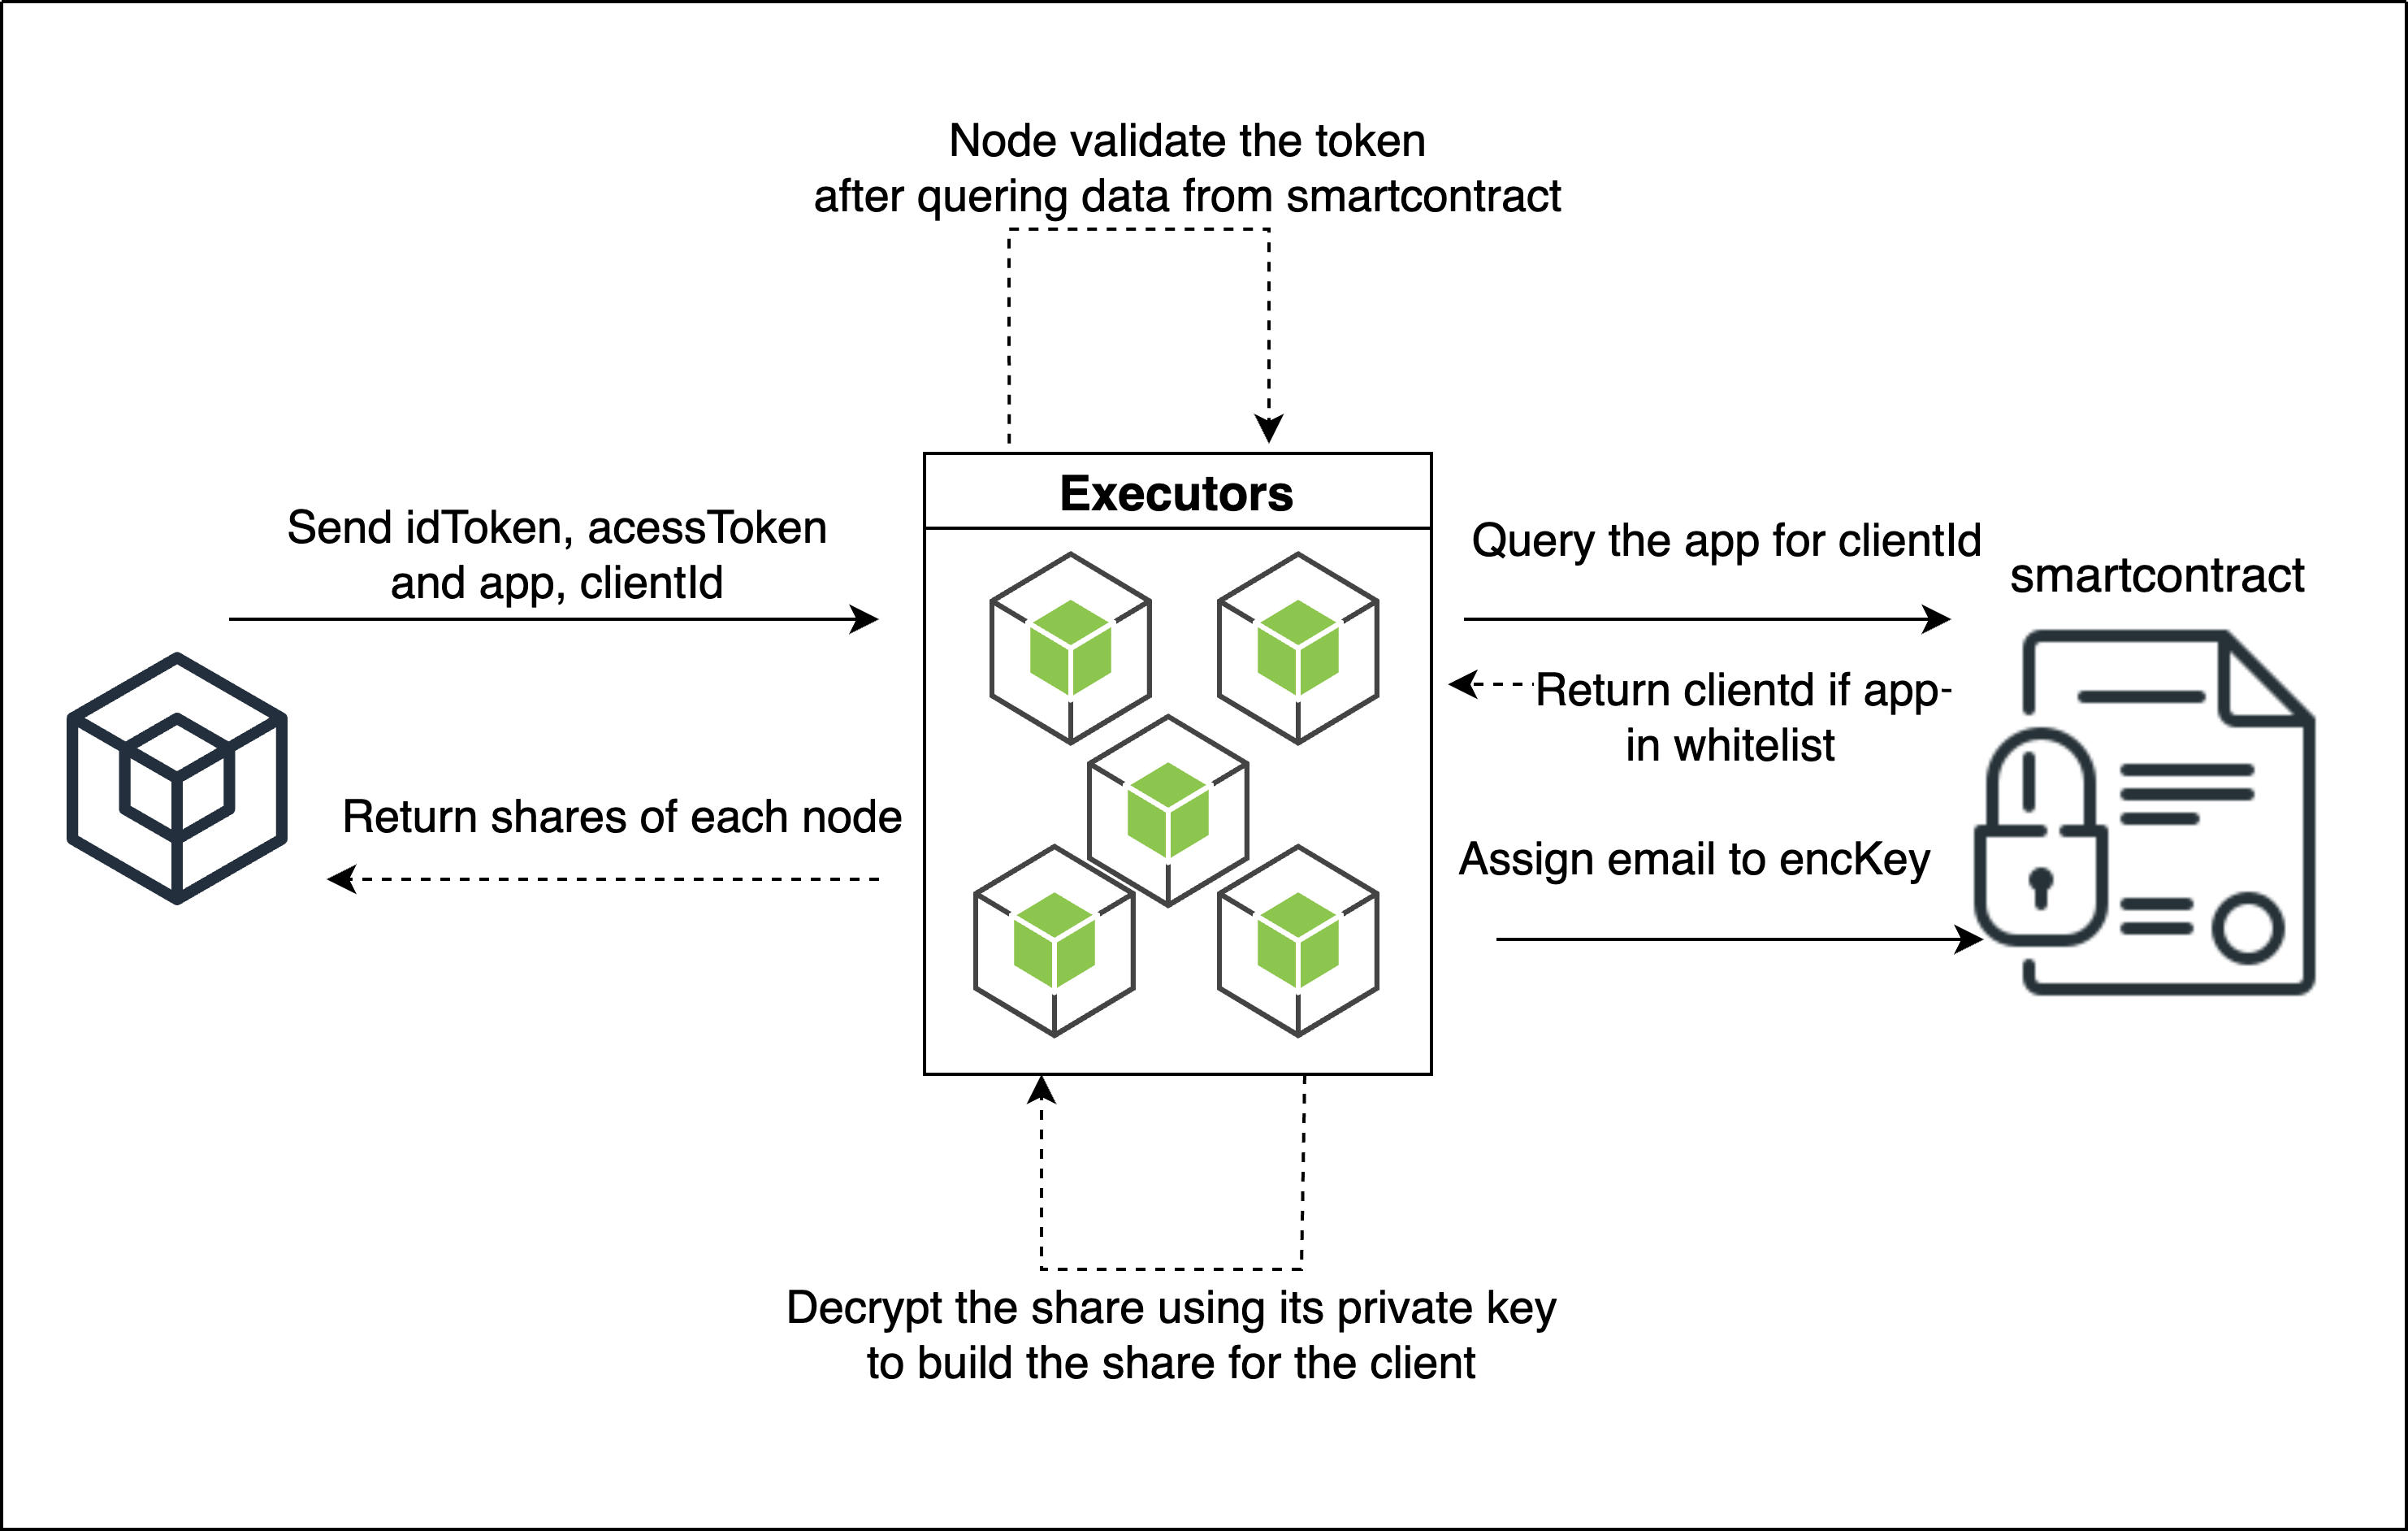
\includegraphics[scale=0.14]{Figure/request-share.png}
    \caption{Request assign the share}
    \label{fig:request-share}
\end{figure}
The process of ensuring secure and effective authentication and authorization in the system, as depicted in Figure \ref{fig:request-share}, consists of multiple phases working in concert to provide a seamless user experience. The SDK, which functions as the interface between the user's device and the system, is central to this process. The SDK transmits the idToken or accessToken, along with the appName and clientId, to the executors whenever the user initiates the authentication process. As essential system components, the executors play a crucial role in authenticating the user's credentials and ensuring secure smart contract interaction. They begin by querying the smart contract to retrieve the app's essential authentication and authorization parameters and configuration data. This data is essential for establishing a secure and trusted connection between the user and the application. Executors initiate the validation procedure after receiving the data from the smart contract. It is essential to validate the integrity and authenticity of the data extracted from the idToken or accessToken to ensure that the user's credentials have not been altered during transmission and are valid. When a new user attempts authentication, the executors generate a unique key for that user. This key functions as a digital identifier and is securely associated with the user's authenticated email address. This phase ensures that each user within the system has a unique and distinguishable key, allowing for secure and efficient user management. The smart contract encrypts the shares using the private keys of the nodes that participated in the protocol as part of the distributed key generation process. The encrypted shares are transmitted in a secure manner to the executors, who can decrypt them with their own private keys. This secure decryption safeguards the shares' confidentiality and integrity, preventing unauthorized access. The executors reconstruct the final share and promptly return it to the SDK after decrypting the shares. These shares play a crucial role in the subsequent phases of authentication and authorization, enabling the user to access and interact with decentralized applications (DApps) within the ecosystem with confidence and security. By strictly adhering to this exhaustive and complex procedure, the system guarantees that user authentication and authorization are both effective and secure. The combination of smart contracts, Shamir secret sharing, and the Pedersen DKG protocol enables the system to offer a robust, trustworthy, and user-friendly Web3 authentication solution. This comprehensive strategy addresses the complexities of Web3 technologies and promotes widespread adoption and utility by improving the security, accessibility, and overall user experience of decentralized applications.
\subsection{Generating and Storing Shares in Metadata}
\begin{figure}[H]
 \centering
 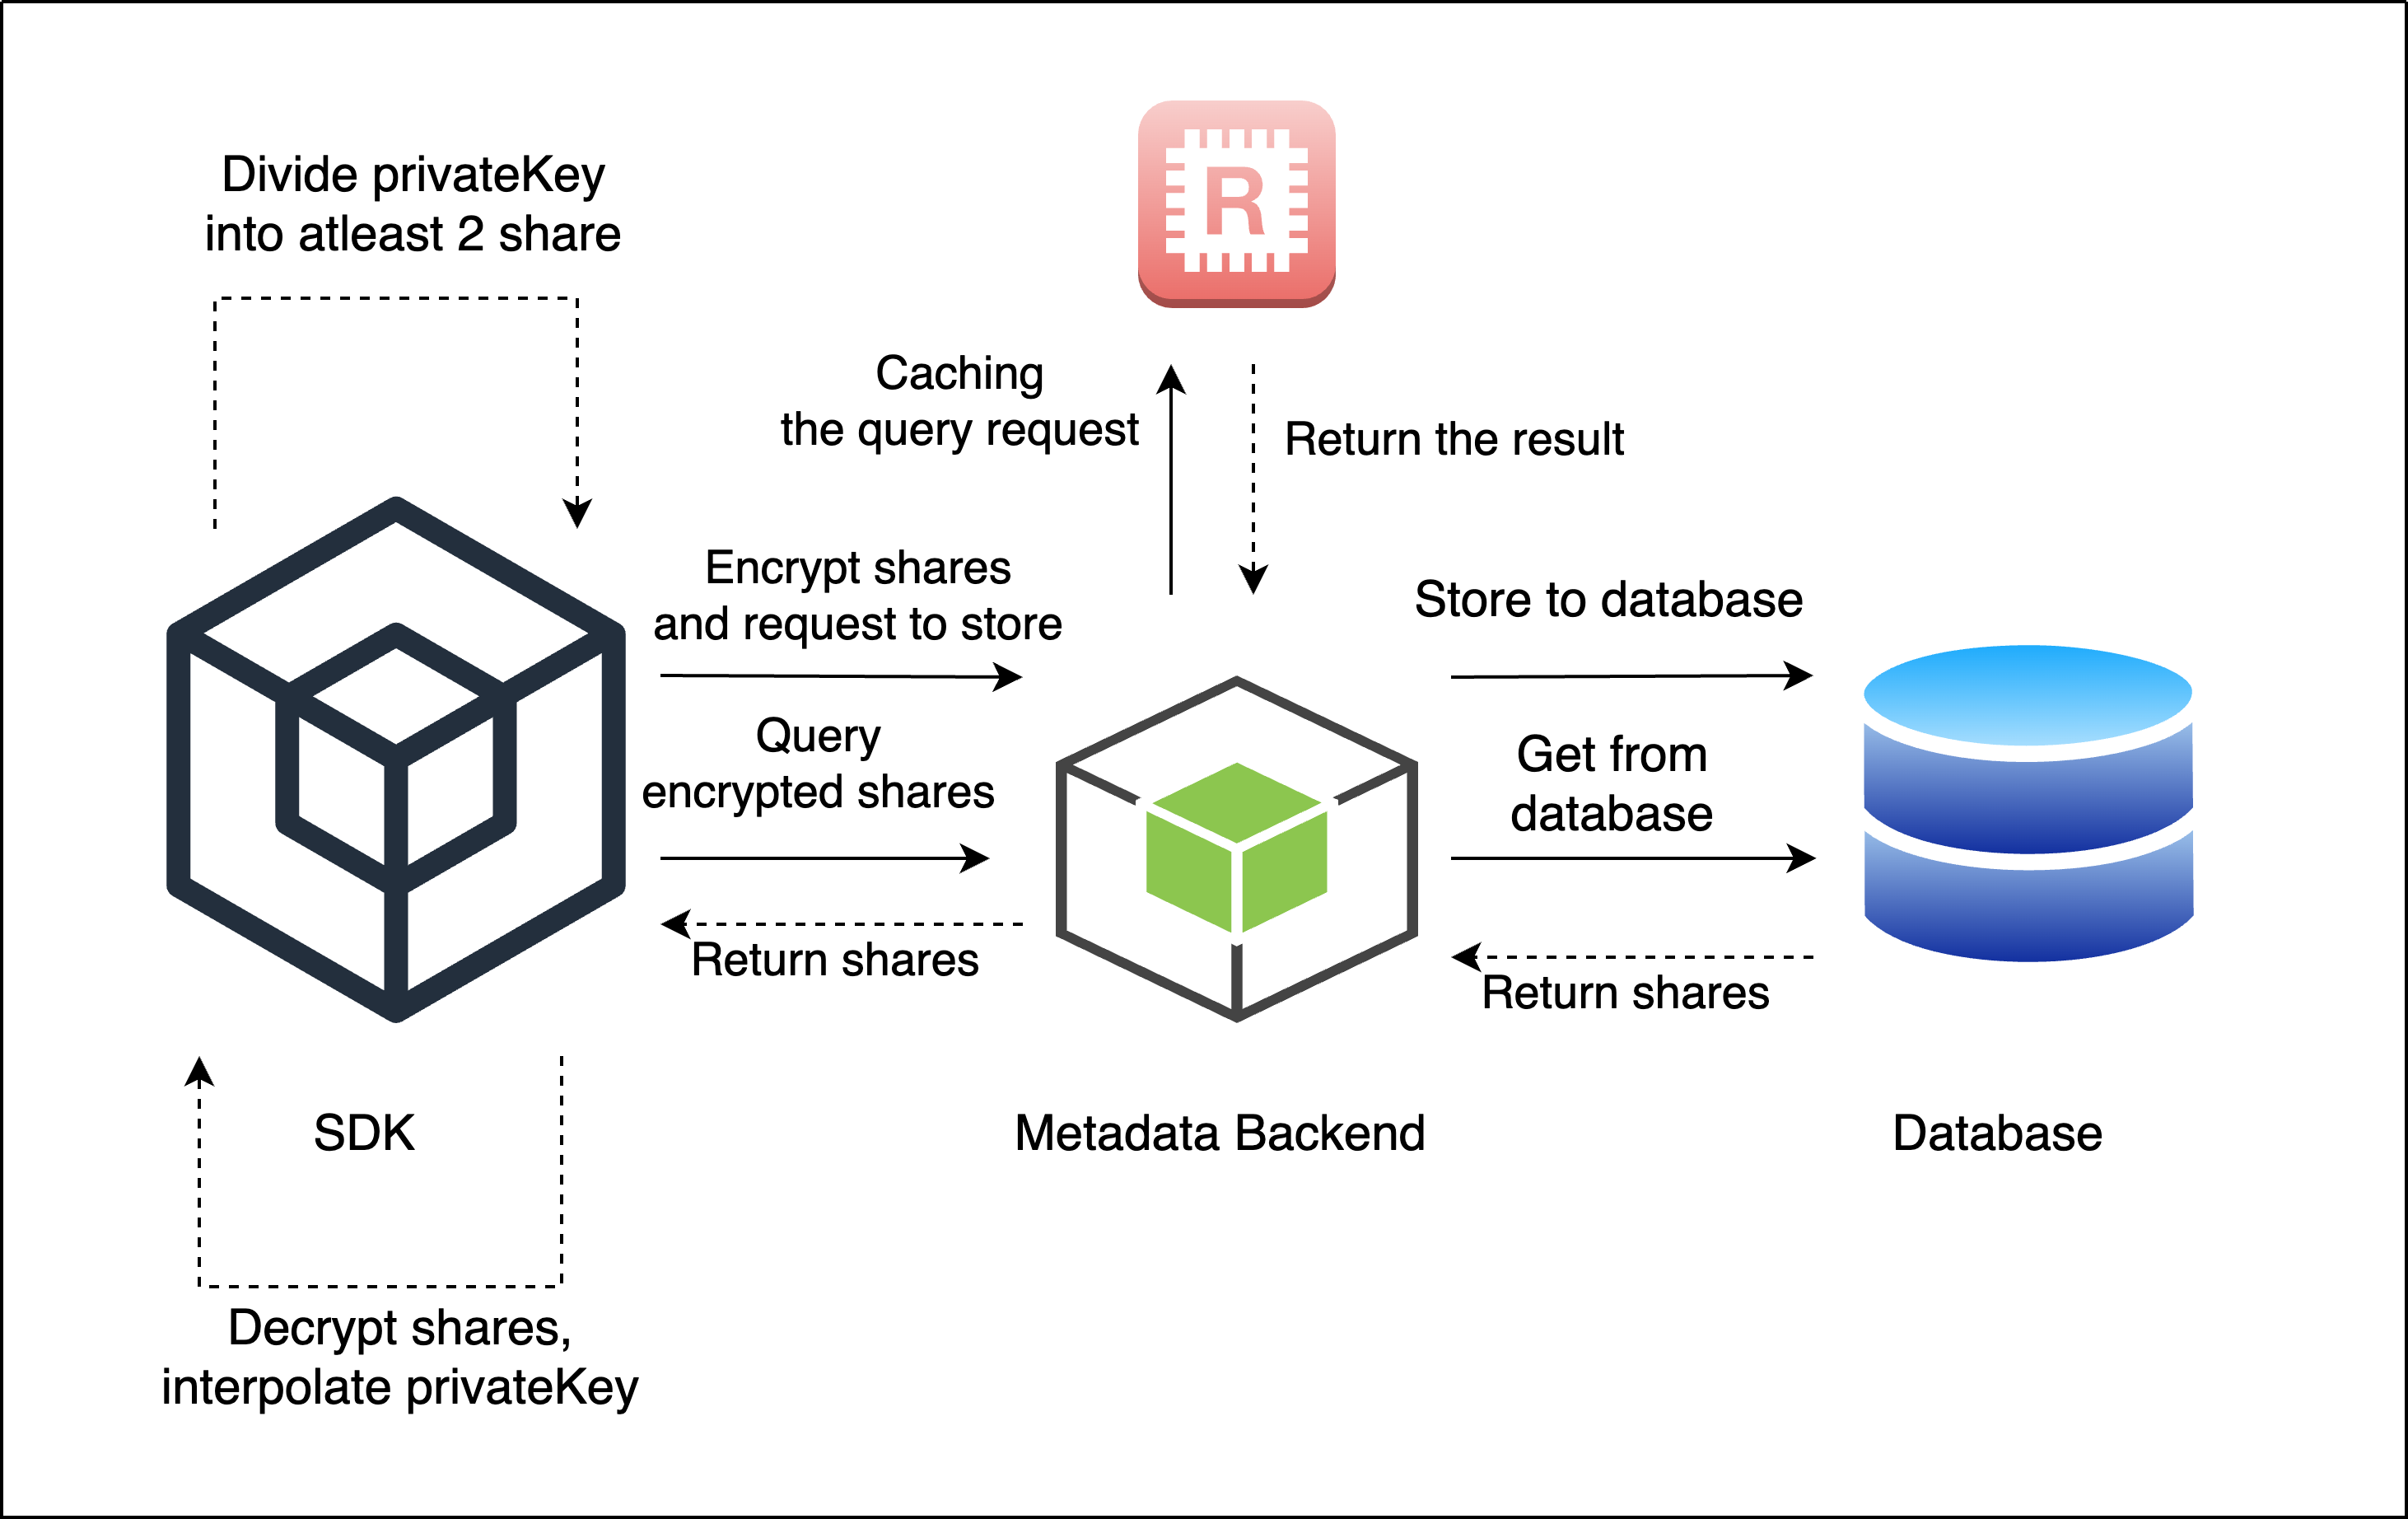
\includegraphics[scale=0.14]{Figure/generate-share.png}
 \caption{Generate & Reconstruct shares}
    \label{fig:generate-share}
\end{figure}
As depicted in \ref{fig:generate-share}, the process of reconstructing the private key in our system consists of multiple phases that have been meticulously designed to ensure optimum security and dependability. It commences with the implementation of Shamir's secret sharing scheme, in which the SDK divides the private key into at least two shares. Each share is then encrypted to ensure its confidentiality and integrity, preventing unauthorized access. These encrypted shares are transmitted in a secure manner to the metadata repository, where they are stored in a database. The SDK initiates a query request to the metadata repository whenever the need arises to reconstruct the private key. The backend retrieves the encrypted shares associated with the specified user and application from the database upon receiving the query. The query result, including the encrypted shares, is cached in a Redis database to boost performance and accelerate subsequent requests. After receiving the encrypted shares, the SDK initiates the reconstruction process. The SDK decrypts each share using its respective decryption key. Only authorized processes have access to these decryption keys, which are managed securely within the SDK. The SDK recovers the original confidential information contained within each share by decrypting the shares. The SDK combines the decrypted shares using interpolation algorithms, such as Lagrange interpolation, to generate the final private key. Using the available shares, this mathematical calculation interpolates the absent portions of the private key. The SDK successfully reconstructs the original private key through this procedure. Throughout the entirety of the reconstruction process, robust encryption algorithms and secure key management procedures are used to protect the privacy and integrity of the private key. The implementation of Shamir's scheme for secret sharing is essential for enhancing security because it distributes the key across multiple shares, making it resistant to single points of failure or compromise. Our system guarantees the safety and reliability of the private key's retrieval by implementing this exhaustive and secure reconstruction procedure. This feature enables users to securely access their Web3 ecosystem accounts and confidently execute authorized operations. In addition, the comprehensive security measures ensure that the private key remains protected and inaccessible to unauthorized entities, giving users peace of mind when interacting with decentralized applications (DApps) and the broader Web3 ecosystem. This procedure's meticulous design and execution exemplify the system's dedication to providing a secure and user-friendly Web3 authentication solution.
\section{Asynchronous create encKey process}
\begin{figure}[H]
 \centering
 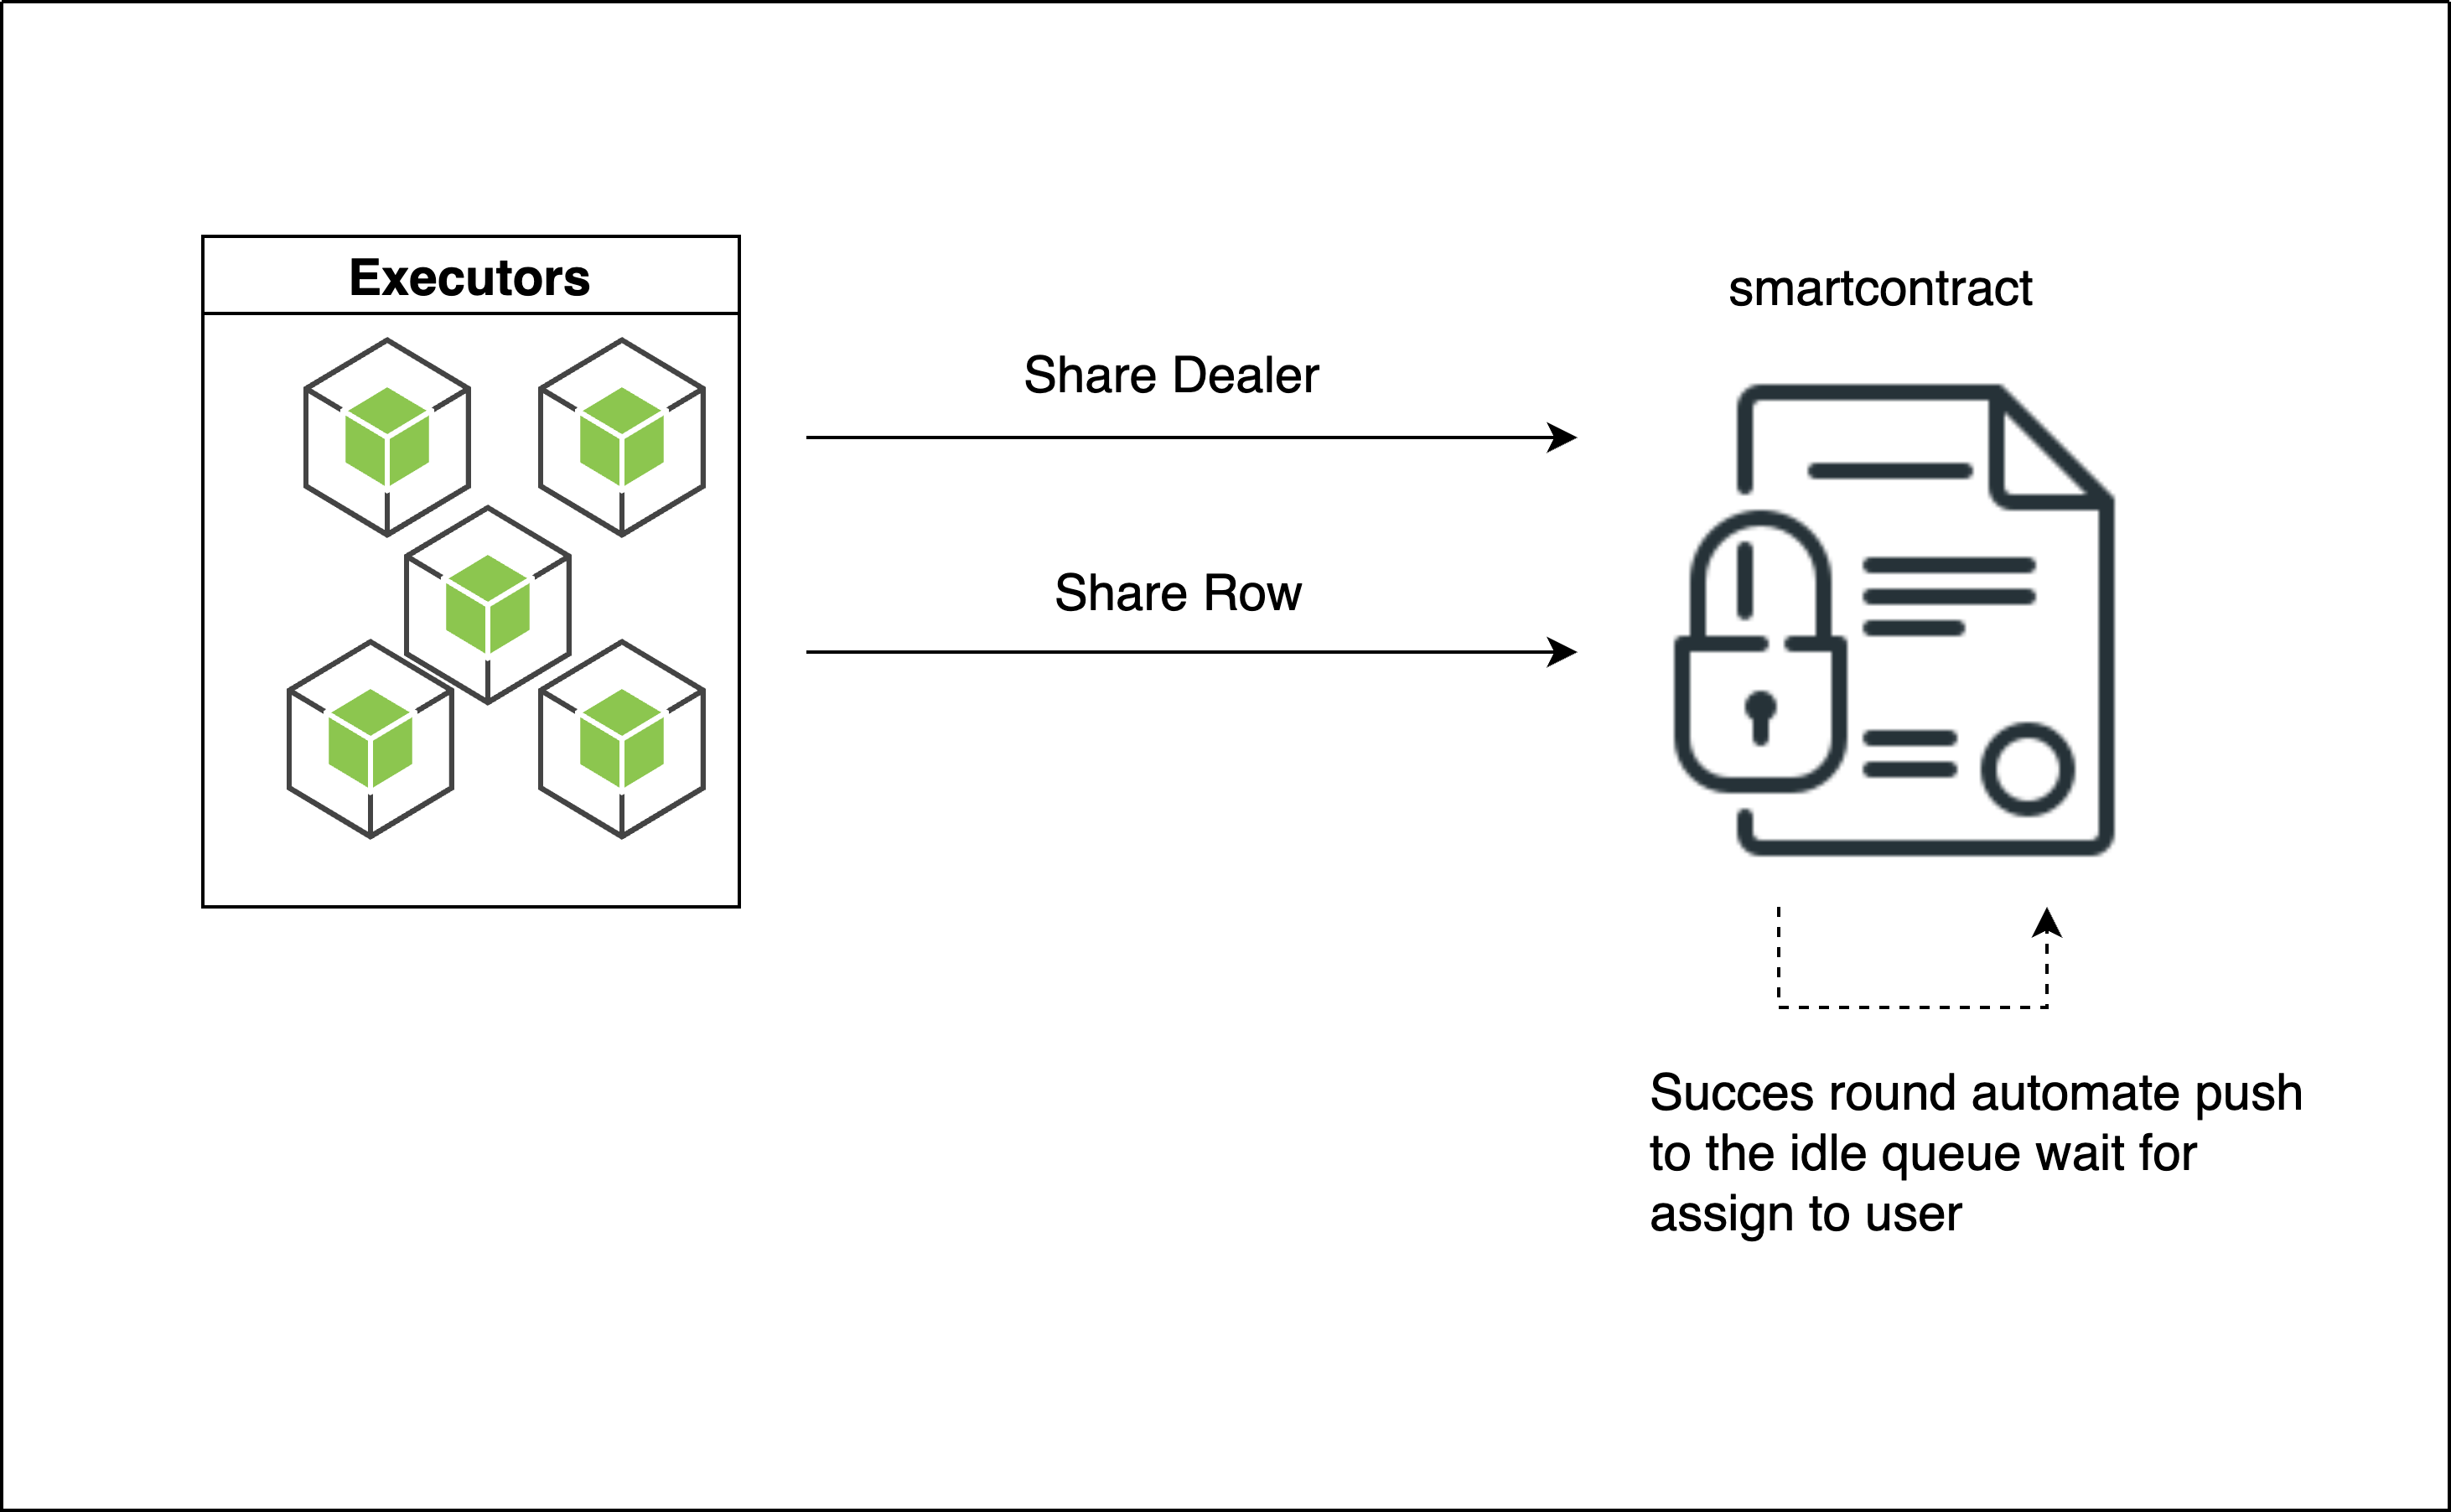
\includegraphics[scale=0.14]{Figure/executor-contribute.png}
 \caption{Asynchronous create encKey}
    \label{fig:create-encKey}
\end{figure}
The asynchronous creation of the encKey process is a crucial and ingenious element of the system's architecture, as it is intended to maximize efficiency and resource utilization. Without running the Distributed Key Generation (DKG) protocol each time, this method ensures that keys can be assigned to users quickly and seamlessly, without the need to run the protocol each time. By generating a pool of unused encKeys in advance, the system significantly reduces the time and computational overhead required for key assignment, ultimately augmenting the user experience. The executors, the pillars of the encKey generation procedure, are responsible for initiating the procedure. They constantly monitor the current round's status and the number of inactive keys. When the system detects a need for new keys, such as when the present state is null or in the "waitfordealer" phase, and the number of idle keys falls below the anticipated threshold, the executors initiate the subsequent round. This proactive strategy ensures that the system is always ready to meet user demands and minimizes any potential delays in key assignment. During the initial phase of the round, known as the "sharing dealer" phase, the executors combine and distribute their individual confidential shares to the designated sharing dealer. This strategic partnership permits each executor to contribute to the procedure without disclosing sensitive information that could compromise the overall secret key. By effectively sharing their secret shares, the executors disseminate the secret in a manner that maintains the keys' security and integrity. Once the "sharing dealer" phase is effectively completed, the protocol seamlessly transitions to the "waitforrows" phase. In this phase, the executors generate their own public key shares using the shared secrets obtained in the previous phase. These public key exchanges are essential to the conclusion of the key generation process, as they guarantee the authenticity and validity of the user-assigned keys. The system is now well-prepared for the assignment of encKeys to users, as the "waitforrows" phase has concluded. When a user requests their key, the system assigns the correct round to their assigned key and provides it, ensuring a speedy and efficient assignment. By adopting this asynchronous method for encKey generation, the system obtains a number of substantial benefits. First, it optimizes resource usage by eliminating the needless re-execution of the DKG protocol for each key assignment. Second, it improves the scalability and performance of the system, allowing it to manage a large number of user requests without compromising response times. Lastly, it assures a secure and seamless workflow for encKey generation and assignment, reinforcing the system's dedication to user convenience and data security. In conclusion, the incorporation of the DKG protocol and the effectiveness of the asynchronous encKey creation procedure demonstrate the innovative and sophisticated nature of the system's design. The system's ability to efficiently generate and assign encKeys contributes to its overall robustness, allowing Web3 ecosystem users to enjoy a secure and user-friendly experience.


\end{document}
